% Papel: A4 – cor branca
% Fonte: Times New Roman ou Arial- tamanho 12 – cor: preta. Nas citações com mais de 3 linhas, notas de rodapé, legendas e tabelas a fonte deve ter o tamanho 10.
% Itálico: Deve ser usado nas palavras de outros idiomas. Esta orientação não se aplica às expressões latinas apud e et al.
% Margens: Direita e inferior: 2cm / Esquerda e superior: 3cm
% Parágrafos / Espaçamento: 1,5 entre linhas;

\documentclass[a4paper,12pt,openany,oneside]{abntex2}
\usepackage[brazil]{babel}
\usepackage[utf8]{inputenc}
\usepackage[T1]{fontenc}

\usepackage[brazil,hyperpageref]{backref}
\usepackage[alf,bibjustif]{abntex2cite}
\usepackage{indentfirst}
\usepackage{microtype}

\usepackage{mathptmx}
\usepackage{url}
\usepackage{dsfont}
\usepackage{lmodern}
\usepackage{ragged2e}
\usepackage{amssymb}
\usepackage{amsmath}
\usepackage{multirow}
\usepackage{colortbl}
\usepackage{xcolor}
\usepackage{graphicx}
\usepackage{booktabs}
\usepackage{pdflscape}
% \usepackage{changepage}
\usepackage{caption}
\usepackage{subcaption}

\usepackage{geometry}
\newgeometry{left=3cm,right=2cm,top=3cm,bottom=2cm}

%%% UFRN
% Padrão dos algoritmos
\usepackage{algorithm}
% \usepackage{algorithmic}
% \usepackage{algorithmicx}
\usepackage{algpseudocode}
%
\usepackage{xpatch}
\makeatletter
\xpatchcmd{\algorithmic}{\itemsep\z@}{\itemsep=-4pt}{}{}
\makeatother
%
\makeatletter
\newenvironment{breakablealgorithm}
{% \begin{breakablealgorithm}
\begin{center}
 \refstepcounter{algorithm}% New algorithm
 \hrule height.8pt depth0pt \kern2pt% \@fs@pre for \@fs@ruled
 \renewcommand{\caption}[2][\relax]{% Make a new \caption
   {\raggedright\textbf{\ALG@name~\thealgorithm} ##2\par}%
   \ifx\relax##1\relax % #1 is \relax
     \addcontentsline{loa}{algorithm}{\protect\numberline{\thealgorithm}##2}%
   \else % #1 is not \relax
     \addcontentsline{loa}{algorithm}{\protect\numberline{\thealgorithm}##1}%
   \fi
   \kern2pt\hrule\kern2pt
 }
}{% \end{breakablealgorithm}
 \kern2pt\hrule\relax% \@fs@post for \@fs@ruled
\end{center}
}
\renewcommand*{\ALG@name}{Algoritmo}
\makeatother
%
\usepackage{setspace}
\let\Algorithm\algorithm
\renewcommand\algorithm[1][]{\Algorithm[#1]\setstretch{0.5}}
%
\renewcommand{\listalgorithmname}{Lista de algoritmos}
\let\oldlistofalgorithms\listofalgorithms
\let\oldnumberline\numberline%
\newcommand{\algnumberline}[1]{Algoritmo~#1 -- }
\renewcommand{\listofalgorithms}{%
  \let\numberline\algnumberline%
  \oldlistofalgorithms
  \let\numberline\oldnumberline%
}
\usepackage{parskip}
\usepackage{etoolbox}
\makeatletter
\patchcmd{\@chapter}
  {\addtocontents{loa}}
  {\addtocontents{loa}{\protect\addvspace{0pt}}}
  {}{}
\makeatother
% Declaracoes em Português
\algrenewcommand\algorithmicend{\textbf{fim}}
\algrenewcommand\algorithmicdo{\textbf{faça}}
\algrenewcommand\algorithmicwhile{\textbf{enquanto}}
\algrenewcommand\algorithmicfor{\textbf{para}}
\algrenewcommand\algorithmicforall{\textbf{para cada}}
\algrenewcommand\algorithmicif{\textbf{se}}
\algrenewcommand\algorithmicthen{\textbf{então}}
\algrenewcommand\algorithmicelse{\textbf{senão}}
\algrenewcommand\algorithmicreturn{\textbf{devolve}}
\algrenewcommand\algorithmicfunction{\textbf{função}}
\algrenewcommand\algorithmicprocedure{\textbf{procedimento}}
\algrenewcommand\algorithmicreturn{\textbf{retorna}}

% Rearranja os finais de cada estrutura
\algrenewtext{EndWhile}{\algorithmicend\ \algorithmicwhile}
\algrenewtext{EndFor}{\algorithmicend\ \algorithmicfor}
\algrenewtext{EndIf}{\algorithmicend\ \algorithmicif}
\algrenewtext{EndFunction}{\algorithmicend\ \algorithmicfunction}

% O comando For, a seguir, retorna 'para #1 -- #2 até #3 faça'
\algnewcommand\algorithmicto{\textbf{até}}
\algrenewtext{For}[3]%
{\algorithmicfor\ #1 $\gets$ #2 \algorithmicto\ #3 \algorithmicdo}


% Lista de abreviaturas
\usepackage{acro}
\DeclareAcronym{ufrn}{
  short = UFRN,
  long = Universidade Federal do Rio Grande do Norte,
  class = abbrev
}

\DeclareAcronym{dimap}{
  short = DIMAp,
  long = Departamento de Informática e Matemática Aplicada,
  class = abbrev
}

\newlist{acronyms}{description}{1}
\newcommand*\addcolon[1]{\normalfont #1 --}
\setlist[acronyms]{labelwidth=0em,leftmargin =0em,noitemsep,itemindent=0pt,font=\addcolon}
\DeclareAcroListStyle{dimap}{list}{list=acronyms}
\acsetup{list-style=dimap}
\acsetup{first-style=short}
\acsetup{hyperref=true}
\acsetup{page-name=Abreviações}
% Lista de símbolos
\DeclareAcronym{lambda}{
  short = $\lambda$,
  long = (Algum símbolo),
  class = symbols
}

%%% Correções
% Sumário
\addtolength{\cftlastnumwidth}{-2em} % Editar de acordo com o indice de maior enumeração
\cftsetindents{part}{0em}{\cftlastnumwidth}
\cftsetindents{chapter}{0em}{\cftlastnumwidth}
\cftsetindents{section}{0em}{\cftlastnumwidth}
\cftsetindents{subsection}{0em}{\cftlastnumwidth}
\cftsetindents{subsubsection}{0em}{\cftlastnumwidth}
\cftsetindents{paragraph}{0em}{\cftlastnumwidth}
\cftsetindents{subparagraph}{0em}{\cftlastnumwidth}
\renewcommand{\cftsubsectionfont}{\normalfont\normalsize}
\renewcommand{\cftsubsubsectionfont}{\normalfont\small}
% Espaçamento do paragráfo
\setlength{\parindent}{1.25cm}
% Fonte da legenda
\captionsetup{font=sf}
% Fonte dos capítulos
\renewcommand{\ABNTEXchapterfont}{\rmfamily\bfseries\selectfont}
% URL links
\hypersetup{pageanchor=false, colorlinks=true, linkcolor=black, citecolor=black, urlcolor=black}
% Cabeçalhos
\renewcommand{\textual}{\pagestyle{abntchapfirst}\aliaspagestyle{chapter}{abntchapfirst}}
% Autoref
\renewcommand{\partautorefname}{Parte}
\renewcommand{\appendixautorefname}{Apêndice}
\renewcommand{\chapterautorefname}{Capítulo}
\renewcommand{\sectionautorefname}{\uppercase{S}eção}
\renewcommand{\subsectionautorefname}{\uppercase{S}ubseção}
\renewcommand{\subsubsectionautorefname}{\uppercase{S}ubsubseção}
\renewcommand{\figureautorefname}{Figura}
\renewcommand{\tableautorefname}{Tabela}
\renewcommand{\equationautorefname}{Equação}
\newcommand{\algorithmautorefname}{Algoritmo}
\renewcommand{\FancyVerbLineautorefname}{Linha}
\renewcommand{\theoremautorefname}{Teorema}
\renewcommand{\pageautorefname}{Página}
\addto\extrasbrazil{
  \def\sectionautorefname{Seção}
  \def\subsectionautorefname{Subseção}
  \def\subsubsectionautorefname{Subsubseção}
}
% Fix counter
\usepackage{chngcntr}
\counterwithin{figure}{chapter}
\counterwithin{table}{chapter}
\counterwithin{equation}{chapter}
\counterwithin{algorithm}{chapter}
% Remove warnings
\pdfstringdefDisableCommands{\let\uppercase\relax}
%%%

\usepackage{titling}
\title{Título do Trabalho}
\author{Nome do(a) author(a)}
\newcommand{\fltitle}{Título do trabalho (em língua estrangeira)}
\newcommand{\advisor}{Titulação e nome do(a) orientador(a)}
\newcommand{\coadvisor}{Titulação e nome do(a) co-orientador(a)}
\renewcommand{\local}{Natal - RN}
\renewcommand{\date}{Data}
\newcommand{\approvaldate}{Data}


\begin{document}

\frontmatter % = \pretextual
\frenchspacing

\pagenumbering{roman}

\begin{center}

\begin{minipage}{2cm}
    \begin{center}
    
\includegraphics[width=1.7cm, height=2.0cm]{frontmatter/images/brasao-ufrn.png}
    \end{center}
\end{minipage}
\begin{minipage}{11cm}
    \begin{center}
        \begin{SingleSpace}
        \textsc{ \small
        Universidade Federal do Rio Grande do Norte\\
        Centro de Ciências Exatas e da Terra\\
        Departamento de Informática e Matemática Aplicada\\
        Bacharelado em Ciência da Computação }
        \end{SingleSpace}
    \end{center}
\end{minipage}
\begin{minipage}{2cm}
    \begin{center}
    
\includegraphics[width=1.8cm, height=1.5cm]{frontmatter/images/logo-dimap.png}
    \end{center}
\end{minipage}

\vfill

{\setlength{\baselineskip} {1.3\baselineskip}
{\LARGE \textbf{\thetitle}}\par}

\vfill

{\large \textbf{\theauthor}}

\vfill

\local \\ \date

\end{center}
\begin{center}

\textbf{\large \theauthor}

\vfill

\textbf{\Large \thetitle}

\vfill

\begin{SingleSpace}
\begin{adjustwidth}{.51\textwidth}{0cm}
\noindent \justify Monografia de Graduação apresentada ao Departamento de
Informática e Matemática Aplicada do Centro de Ciências Exatas e da Terra da
Universidade Federal do Rio Grande do Norte como requisito parcial para a obtenção
do grau de bacharel em Ciência da Computação.
\end{adjustwidth}
\end{SingleSpace}

\vfill

Orientador(a)\\ \advisor

\vspace{0.8cm}

Co-orientador(a)\\ \coadvisor

\vfill

\begin{SingleSpace}
\textsc{Universidade Federal do Rio Grande do Norte -- UFRN\\
Departamento de Informática e Matemática Aplicada -- DIMAp }
\end{SingleSpace}

\vfill

\local \\ \date

\end{center}
\begin{folhadeaprovacao}
    \noindent Monografia de Graduação sob o título \textit{\thetitle} apresentada por \theauthor e aceita pelo Departamento de Informática e Matemática Aplicada do Centro de Ciências Exatas e da Terra da Universidade Federal do Rio Grande do Norte, sendo aprovada por todos os membros da banca examinadora abaixo especificada:
    
    \vfill
    
    \setlength{\ABNTEXsignthickness}{0.4pt}
    \setlength{\ABNTEXsignwidth}{10cm}
    \setlength{\ABNTEXsignskip}{2.5cm}
    
    \assinatura{\advisor\\
    {\small Orientador(a)} \\
    {\footnotesize
    Departamento\\
    Universidade}
    }
    
    \assinatura{\coadvisor \\
    {\small Co-orientador(a)} \\
    {\footnotesize
    Departamento\\
    Universidade}
    }
    
    \assinatura{Titulação e nome do membro da banca examinadora \\
    {\footnotesize
    Departamento\\
    Universidade}
    }
    
    \assinatura{Titulação e nome do membro da banca examinadora \\ 
    {\footnotesize
    Departamento \\
    Universidade}
    }
    
    \vfill
    
    \begin{center}
    \local, \approvaldate.
    \end{center}
\end{folhadeaprovacao}


\begin{dedicatoria}

~\vfill

\begin{flushright}
À minha família e amigos.
\end{flushright}

\vspace{5cm}~

\end{dedicatoria}
\begin{agradecimentos}
Agradecimentos dirigidos àqueles que contribuíram de maneira relevante à elaboração do trabalho, sejam eles pessoas ou mesmo organizações.
\end{agradecimentos}

\begin{epigrafe}

~\vfill

\begin{flushright}
\textit{Citação}\medskip\\
Autor
\end{flushright}

\vspace{5cm}~

\end{epigrafe}


\renewcommand{\thepage}{\roman{page}}
\setcounter{page}{1}

% Resumo em língua vernácula
\begin{center}
{\Large{\textbf{\thetitle}}}
\end{center}

\vspace{1cm}

\begin{flushright}
Autor: \theauthor\\
Orientador(a): \advisor\\
Co-orientador(a): \coadvisor
\end{flushright}

\vspace{1cm}

\begin{center}
	\Large{\textsc{\textbf{Resumo}}}
\end{center}

% De 150 à 500 palavras
\noindent O resumo deve apresentar de forma concisa os pontos relevantes de um texto, fornecendo uma visão rápida e clara do conteúdo e das conclusões do trabalho. O texto, redigido na forma impessoal do verbo, é constituído de uma seqüência de frases concisas e objetivas e não de uma simples enumeração de tópicos, não ultrapassando 500 palavras, seguido, logo abaixo, das palavras representativas do conteúdo do trabalho, isto é, palavras-chave e/ou descritores. Por fim, deve-se evitar, na redação do resumo, o uso de parágrafos (em geral resumos são escritos em parágrafo único), bem como de fórmulas, equações, diagramas e símbolos, optando-se, quando necessário, pela transcrição na forma extensa, além de não incluir citações bibliográficas.
\vspace{\onelineskip}

\noindent\textit{Palavras-chave}: Palavra-chave 1, Palavra-chave 2, Palavra-chave 3.
\begin{center}
\Large \textbf{\fltitle}
\end{center}

\vspace{1cm}

\begin{flushright}
Author: Nome do(a) aluno(a)\\
Advisor: \advisor\\
Co-advisor: \coadvisor
\end{flushright}

\vspace{1cm}

\begin{center}
	\Large{\textsc{\textbf{Abstract}}}
\end{center}

\noindent O resumo em língua estrangeira (em inglês \textit{Abstract}, em espanhol \textit{Resumen}, em francês \textit{Résumé}) é uma versão do resumo escrito na língua vernácula para idioma de divulgação internacional. Ele deve apresentar as mesmas características do anterior (incluindo as mesmas palavras, isto é, seu conteúdo não deve diferir do resumo anterior), bem como ser seguido das palavras representativas do conteúdo do trabalho, isto é, palavras-chave e/ou descritores, na língua estrangeira. Embora a especificação abaixo considere o inglês como língua estrangeira (o mais comum), não fica impedido a adoção de outras linguas (a exemplo de espanhol ou francês) para redação do resumo em língua estrangeira.
\vspace{\onelineskip}

\noindent\textit{Keywords}: Keyword 1, Keyword 2, Keyword 3.

% Lista de figuras
\pdfbookmark[0]{\listfigurename}{lof}
\listoffigures
\cleardoublepage
% Lista de tabelas
\pdfbookmark[0]{\listtablename}{lot}
\listoftables
\cleardoublepage
% Lista de algoritmos
\listofalgorithms
\addcontentsline{toc}{chapter}{Lista de algoritmos}
\cleardoublepage
% Lista de abreviaturas
\printacronyms[include-classes=abbrev,heading=chapter*,name=Lista de abreviaturas e siglas]
\cleardoublepage
% Lista de símbolos
\printacronyms[include-classes=symbols,heading=chapter*,name=Lista de símbolos]
\cleardoublepage
% Sumário
\pdfbookmark[0]{\contentsname}{toc}
\tableofcontents
\cleardoublepage

\mainmatter % = \textual
\renewcommand{\thepage}{\arabic{page}}
\setcounter{page}{1}

\pagenumbering{arabic}

% Introdução
\chapter{Introdução}

A introdução é a parte inicial do texto e que possibilita uma visão geral de todo o trabalho, devendo constar a delimitação do assunto tratado, objetivos da pesquisa, motivação para o desenvolvimento da mesma e outros elementos necessários para situar o tema do trabalho.

\section{Organização do trabalho}

Nesta seção deve ser apresentado como está organizado o trabalho, sendo descrito, portanto, do que trata cada capítulo.
% Capítulo 2
\chapter{Capítulo 2}

Este é o primeiro capítulo da parte central do trabalho, isto é, o desenvolvimento, a parte mais extensa de todo o trabalho. Geralmente o desenvolvimento é dividido em capítulos, cada um com subseções e subseções, cujo tamanho e número de divisões variam em função da natureza do conteúdo do trabalho.

Em geral, a parte de desenvolvimento é subdividida em quatro subpartes:
\begin{itemize}
	\item \textit{contextualização ou definição do problema} -- consiste em descrever a situação ou o contexto geral referente ao assunto em questão, devem constar informações atualizadas visando a proporcionar maior consistência ao trabalho;
	\item \textit{referencial ou embasamento teórico} -- texto no qual se deve apresentar os aspectos teóricos, isto é, os conceitos utilizados e a definição dos mesmos; nesta parte faz-se a revisão de literatura sobre o assunto, resumindo-se os resultados de estudos feitos por outros autores, cujas obras citadas e consultadas devem constar nas referências;
	\item \textit{metodologia do trabalho ou procedimentos metodológicos} -- deve constar o instrumental, os métodos e as técnicas aplicados para a elaboração do trabalho;
	\item \textit{resultados} -- devem ser apresentados, de forma objetiva, precisa e clara, tanto os resultados positivos quanto os negativos que foram obtidos com o desenvolvimento do trabalho, sendo feita uma discussão que consiste na avaliação circunstanciada, na qual se estabelecem relações, deduções e generalizações.
\end{itemize}

É recomendável que o número total de páginas referente à parte de desenvolvimento não ultrapasse 60 (sessenta) páginas.

\section{Seção 1}

Teste de figura:

\subsection{Subseção 1.1}

\begin{figure}[htb]
\centering
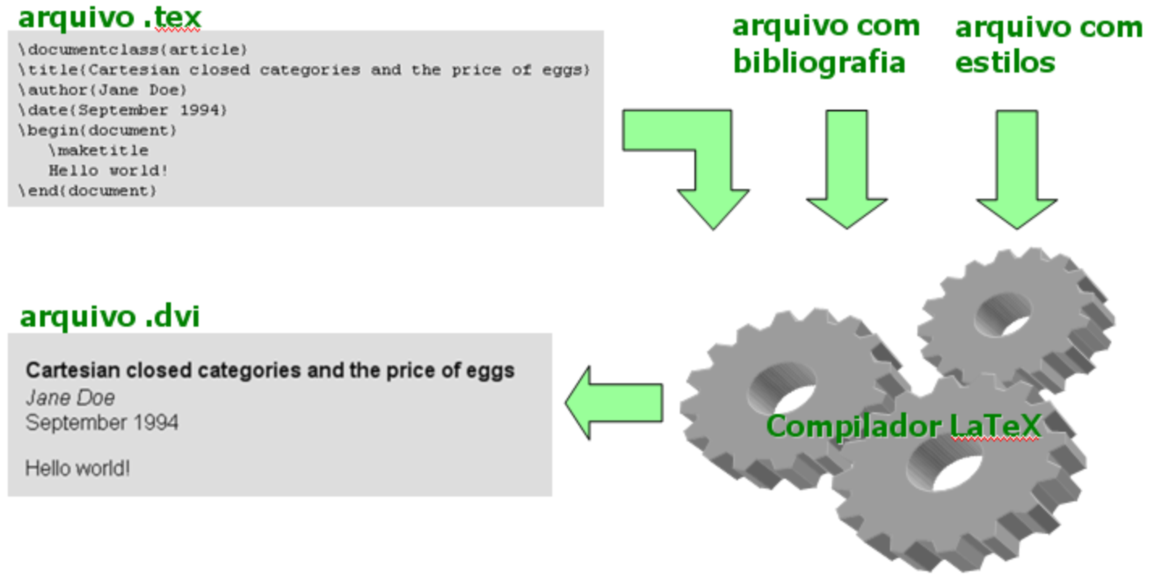
\includegraphics[scale=7.0]{mainmatter/images/figura_teste.png}
\caption{Teste de uma figura em formato .png}
\label{fig:FiguraTeste}
\end{figure}

\begin{figure}[htb]
\centering
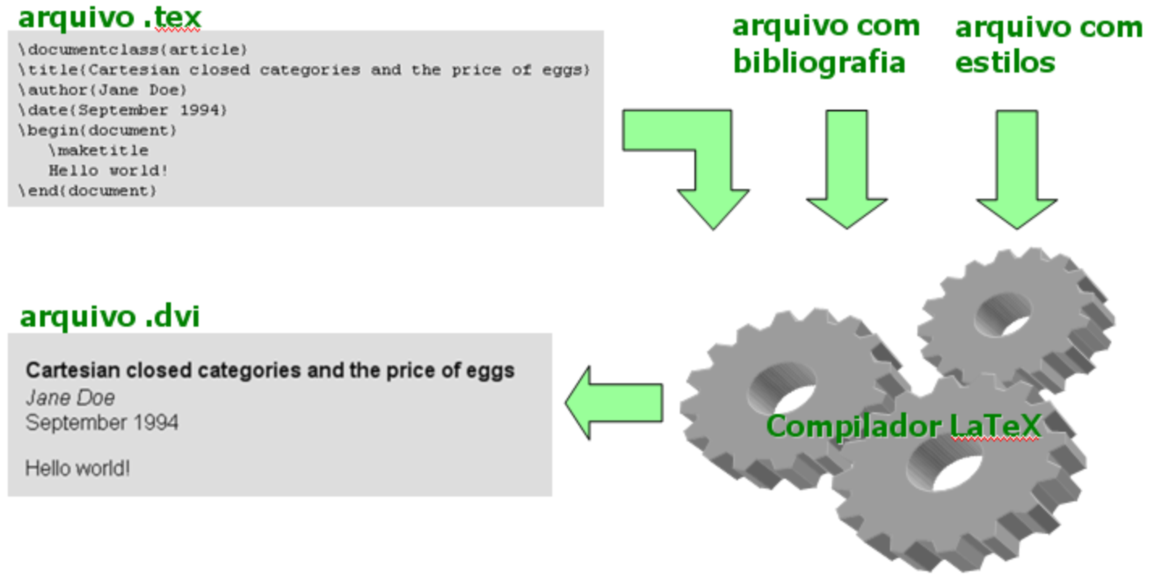
\includegraphics[scale=7.0]{mainmatter/images/figura_teste.png}
\caption{Teste de uma figura em formato .png}
\label{fig:FiguraTeste2}
\end{figure}


\section{Seção 2}

Referenciamento da figura inserida na seção anterior: \autoref{fig:FiguraTeste} na página \pageref{fig:FiguraTeste}

Figura \ref{fig:FiguraTeste}, Figura \ref{fig:FiguraTeste2}, \autoref{fig:FiguraTeste}.

\section{Seção 3}

Seção 3 \ref{fig:FiguraTeste}


\section{Seção 4}

Seção 4
% Capítulo 3
\chapter{Capítulo 3}

Algumas regras devem ser observadas na redação da monografia:
\begin{enumerate}
	\item ser claro, preciso, direto, objetivo e conciso, utilizando frases curtas e evitando ordens inversas desnecessárias;
	\item construir períodos com no máximo duas ou três linhas, bem como parágrafos com cinco linhas cheias, em média, e no máximo oito (ou seja, não construir parágrafos e períodos muito longos, pois isso cansa o(s) leitor(es) e pode fazer com que ele(s) percam a linha de raciocínio desenvolvida);
	\item a simplicidade deve ser condição essencial do texto; a simplicidade do texto não implica necessariamente repetição de formas e frases desgastadas, uso exagerado de voz passiva (como \textit{será iniciado}, \textit{será realizado}), pobreza vocabular etc. Com palavras conhecidas de todos, é possível escrever de maneira original e criativa e produzir frases elegantes, variadas, fluentes e bem alinhavadas;
	\item adotar como norma a ordem direta, por ser aquela que conduz mais facilmente o leitor à essência do texto, dispensando detalhes irrelevantes e indo diretamente ao que interessa, sem rodeios (verborragias);
	\item não começar períodos ou parágrafos seguidos com a mesma palavra, nem usar repetidamente a mesma estrutura de frase;
	\item desprezar as longas descrições e relatar o fato no menor número possível de palavras;
	\item recorrer aos termos técnicos somente quando absolutamente indispensáveis e nesse caso colocar o seu significado entre parênteses (ou seja, não se deve admitir que todos os que lerão o trabalho já dispõem de algum conhecimento desenvolvido no mesmo);
	\item dispensar palavras e formas empoladas ou rebuscadas, que tentem transmitir ao leitor mera idéia de erudição;
	\item não perder de vista o universo vocabular do leitor, adotando a seguinte regra prática: \textit{nunca escrever o que não se diria};
	\item termos coloquiais ou de gíria devem ser usados com \textit{extrema} parcimônia (ou mesmo nem serem utilizados) e apenas em casos muito especiais, para não darem ao leitor a idéia de vulgaridade e descaracterizar o trabalho;
	\item ser rigoroso na escolha das palavras do texto, desconfiando dos sinônimos perfeitos ou de termos que sirvam para todas as ocasiões; em geral, há uma palavra para definir uma situação;
	\item encadear o assunto de maneira suave e harmoniosa, evitando a criação de um texto onde os parágrafos se sucedem uns aos outros como compartimentos estanques, sem nenhuma fluência entre si;
	\item ter um extremo cuidado durante a redação do texto, principalmente com relação às regras gramaticais e ortográficas da língua; geralmente todo o texto é escrito na forma impessoal do verbo, não se utilizando, portanto, de termos em primeira pessoa, seja do plural ou do singular.
\end{enumerate}


\section{Seção 1}

Teste de uma tabela:

\begin{table}[htb]
% Título de tabelas sempre aparecem antes da tabela
\caption{Tabela sem sentido}
\label{tab:TabelaSemSentido}
\center
{
	\begin{tabular}{l|l}
		\hline
		Titulo Coluna 1   & Título Coluna 2\\
		\hline
		X                 & Y\\
		X                 & W\\
		\hline
	\end{tabular}
}
\end{table}


\section{Seção 2}

Seção 2


\subsection{Subseção 2.1}

Referência à tabela definida no início: \ref{tab:TabelaSemSentido}


\subsection{Subseção 2.2}

Subsection 2.2


\section{Seção 3}

Seção 3
% Capítulo 4
\chapter{Capítulo 4}

\section{Seção 1}

Teste para símbolo

\ac{lambda}


\section{Seção 2}

Teste para abreviatura 

\ac{ufrn}

\ac{dimap}


\begin{breakablealgorithm}
\begin{algorithmic}[1]
\If {$i\geq maxval$}
    \State $i\gets 0$
\Else
    \If {$i+k\leq maxval$}
        \State $i\gets i+k$
    \EndIf
\EndIf
\end{algorithmic}
\caption{Esperança}
\label{alg1}
\end{breakablealgorithm}
% Capítulo 5
\chapter{Capítulo 5}

\section{Seção 1}

Seção 1


\section{Seção 2}

Alguns exemplos de citação: 

Na tese de Doutorado de Paquete \cite{PaquetePhD}, discute-se sobre algoritmos de busca local estocásticos aplicados a problemas de Otimização Combinatória considerando múltiplos objetivos. Por sua vez, o trabalho de \cite{KnowlesBoundedLebesgue}, publicado nos anais do IEEE CEC de 2003, mostra uma técnica de arquivamento também empregada no desenvolvimento de algoritmos evolucionários multi-objetivo, trabalho esse posteriormente estendido para um capítulo de livro dos mesmos autores \cite{KnowlesBoundedPareto}. Por fim, no relatório técnico de \citeonline{Jaszkiewicz}, fala-se sobre um algoritmo genético híbrido para problemas multi-critério, enquanto no artigo de jornal de Lopez \textit{et al.} \cite{LopezPaqueteStu} trata-se do \textit{trade-off} entre algoritmos genéticos e metodologias de busca local, também aplicados no contexto multi-critério e relacionado de alguma forma ao trabalho de Jaszkiewicz (\citeyear{Jaszkiewicz}).

Outros exemplos relacionados encontram-se em \cite{Silberschatz} (livro), \cite{DB2XML} (referência da Web) e \cite{Angelo} (dissertação de Mestrado).

\subsection{Subseção 5.1}

Subseção 5.1


\subsection{Subseção 5.2}

Subsection 5.2


\section{Seção 3}

Seção 3
% Considerações finais
\chapter{Considerações finais}

As considerações finais formam a parte final (fechamento) do texto, sendo dito de forma resumida (1) o que foi desenvolvido no presente trabalho e quais os resultados do mesmo, (2) o que se pôde concluir após o desenvolvimento bem como as principais contribuições do trabalho, e (3) perspectivas para o desenvolvimento de trabalhos futuros. O texto referente às considerações finais do autor deve salientar a extensão e os resultados da contribuição do trabalho e os argumentos utilizados estar baseados em dados comprovados e fundamentados nos resultados e na discussão do texto, contendo deduções lógicas correspondentes
aos objetivos do trabalho, propostos inicialmente.

\bibliography{mainmatter/refs}
\bibliographystyle{abntex2-alf}
\bibliographystyle{abntex2-num}


\backmatter % = \postextual

\begin{apendicesenv}
\partapendices
\chapter{Primeiro Apêndice}

Os apêndices são textos ou documentos elaborados pelo autor, a fim de complementar sua argumentação, sem prejuízo da unidade nuclear do trabalho.
\end{apendicesenv}

\begin{anexosenv}
\partanexos
% \annex
\chapter{Primeiro Anexo}

Os anexos são textos ou documentos não elaborado pelo autor, que servem de fundamentação, comprovação e ilustração.
\end{anexosenv}

\end{document}
